\documentclass{beamer}

\usepackage[english]{babel}
\usepackage{amsmath,amsthm,amsfonts}
\usepackage{xkeyval}
\usepackage{graphics}
\usepackage{float}
\usepackage{url,hyperref}
\usepackage{colortbl}%color a table
\usepackage[lined,boxed,linesnumbered]{algorithm2e}
\usepackage{CJKutf8}
\usepackage{multimedia}

\definecolor{mycolor}{RGB}{153,50,204}
\definecolor{mycolorlys}{RGB}{148,0,211}
\definecolor{mycolorlyslys}{RGB}{138,43,226}
\definecolor{mycolorlyslyslys}{RGB}{147,112,219}

\definecolor{color1}{RGB}{132,112,255}
\definecolor{color2}{RGB}{135,206,250}
\definecolor{color3}{RGB}{255,245,238}
\definecolor{color4}{RGB}{255,165,0}
\definecolor{color5}{RGB}{255,20,147}
\definecolor{color6}{RGB}{147,112,219}

%输入罗马数字
\newcommand{\myRoman}[1]{\uppercase\expandafter{\romannumeral#1}}
\newcommand{\myroman}[1]{\romannumeral#1}

\mode<presentation>
{
	\usetheme{Madrid}
	\usecolortheme[named=mycolor]{structure}
	\useinnertheme{rectangles}
	\useoutertheme{infolines}%default,infolines,miniframes,shadow,sidebar,smoothbars,smoothtree,split,tree
	\usefonttheme[onlymath]{serif}
	\setbeamercovered{transparent}
	\setbeamertemplate{blocks}[rounded][shadow=true]
}

\title{Introduction to AdaBoost}
\author{Yunfei WANG\\{\small \url{yunfeiwang@hust.edu.cn}}}
\institute{\inst{1}School of Computer Science \& Technology \\ Huazhong University of Science \& Technology}
\date{October 22, 2013}
%\logo{
\includegraphics[scale=0.07]{images/HUSTLogo}}

\begin{document}
\begin{CJK*}{UTF8}{gbsn}

\begin{frame}
\titlepage
\end{frame}

%\begin{frame}\frametitle{Table of contents}
%\tableofcontents
%\end{frame}


\begin{frame}\frametitle{What's AdaBoost}
\begin{alertblock}{}
\textcolor{cyan}{AdaBoost(adaptive boosting)} is an algorithm for constructing a "strong" classifier as linear combination of "weak" classifiers $h_m(x)\in\{-1,1\}$
\begin{equation}
f(x)=\sum_{m=1}^L\alpha_mh_m(x)
\end{equation}
where $\alpha_m$ is the contribution factor of $h_m(x)$.\\
\medskip
\textcolor{red}{Final classifier: $H(x)=sign(f(x))$.}
\end{alertblock}
\medskip
\begin{block}{}
AdaBoost is adaptive in the sense that subsequent classifiers are chosen in favor of samples misclassified by previous classifiers.
\end{block}
\medskip 
\begin{block}{}
As long as a classifier is slightly better than random, it can improve the final model. Even classifiers with higher error rate will be help, since they'll have negative coefficients and behave like their inverse.
\end{block}
\end{frame}

\begin{frame}\frametitle{Scouting}
Scouting is done by testing each classifier with a training set of $N$ samples $\mathcal{S}=\{(x_1,y_1),(x_2,y_2),\cdots,(x_N,y_N)|y_i\in\{-1,1\}\}$.
\begin{table}
\begin{tabular}{>{\columncolor{color1}}c|>{\columncolor{color2}}c>{\columncolor{color3}}c>{\columncolor{color4}}c>{\columncolor{color5}}c>{\columncolor{color6}}c}
 & $1$ & $2$ & $3$ & $\cdots$ & $L$\\
$x_1$ & $0$ & $0$ & $1$ & $\cdots$ & $1$\\
$x_2$ & $1$ & $0$ & $0$ & $\cdots$ & $0$\\
$x_3$ & $0$ & $1$ & $1$ & $\cdots$ & $0$\\
$\vdots$ & $\vdots$ & $\vdots$ & $\vdots$ & $\ddots$ & $\vdots$\\
$x_N$ & $1$ & $0$ & $0$ & $\cdots$ & $0$\\
\end{tabular}
\caption{Scouting Result of $L$ Classifiers}
\end{table}
\begin{center}
{\textcolor{green}{$0$-Correct}     \textcolor{red}{$1$-Wrong}}
\end{center}
\end{frame}


\begin{frame}\frametitle{Modelling}
At the $m$-th iteration, we have included $m-1$ classifiers, the linear combination of classifiers is
\begin{equation}
f_{m-1}(x)=\alpha_1h_1(x)+\alpha_2h_2(x)+\cdots+\alpha_{m-1}h_{m-1}(x)
\end{equation}
We want to recruit the next classifier
\begin{equation}
f_m(x)=f_{m-1}(x)+\alpha_mh_m(x)
\end{equation}
\begin{exampleblock}{The exponential loss of current classifier $sign(f_m(x))$}
\begin{equation}
\mathcal{L}_m=\sum_{i=1}^Ne^{-y_i(f_{m-1}(x_i)+\alpha_mh_m(x_i))}
\end{equation}
where $\alpha_m$ and $h_m$ are to be determined in an optimal way.
\end{exampleblock}
\end{frame}

\begin{frame}\frametitle{How to choose $h_m$?}
%We rewrite our loss function as
%\begin{equation}
%\mathcal{L}_m=\sum_{i=1}^Nw_i^{(m)}e^{-y_i\alpha_mh_m(x_i)}
%\end{equation}
%where $w_i^{(m)}=e^{-y_if_{m-1}(x_i)}$ is the weight assigned to each sample.
\begin{block}{}
According to the results of classifier $h_m$, we split $\mathcal{L}_m$ into two parts
\begin{equation}
\mathcal{L}_m=\sum_{i:y_i=h_m(x_i)}w_i^{(m)}e^{-\alpha_m}+\sum_{i:y_i\neq h_m(x_i)}w_i^{(m)}e^{\alpha_m}=W_ce^{-\alpha_m}+W_ee^{\alpha_m}
\end{equation}
where $w_i^{(m)}=e^{-y_if_{m-1}(x_i)}$ is the weight assigned to each sample.
\end{block}
\begin{alertblock}{}
When selecting $h_m$, we change the form of \(\mathcal{L}_m\)
\begin{equation}
\mathcal{L}_m=(W_c+W_e)e^{-\alpha_m}+W_e(e^{\alpha_m}-e^{-\alpha_m})
\end{equation}
$W=W_c+W_e$ is the sum of weights of all samples, which is fixed in current iteration. We'll choose the classifier with lowest $W_e(\alpha_m>0)$ or highest $W_e(\alpha_m<0)$.
\end{alertblock}
\end{frame}


\begin{frame}\frametitle{What is the optimal $\alpha_m$ for $h_m$?}
Having picked the $m$-th classifier, we need to determine its weight $\alpha_m$
\begin{equation}
\frac{\partial\mathcal{L}_m}{\partial\alpha_m}=-W_ce^{-\alpha_m}+W_ee^{\alpha_m}
\end{equation}
Setting the partial derivative to zero and rescaling it by $e^{\alpha_m}$
\begin{equation}
-W_c+W_ee^{2\alpha_m}=0
\end{equation}
\begin{exampleblock}{The optimal $\alpha_m$ is thus}
\begin{equation}
\alpha_m=\frac{1}{2}log(\frac{W_c}{W_e})=\frac{1}{2}log(\frac{W-W_e}{W_e})=\frac{1}{2}log(\frac{1-\epsilon_m}{\epsilon_m})
\end{equation}
where $\epsilon_m=W_c/W_e$ is the rate of error given the weights of all samples.
\end{exampleblock}
\end{frame}

\begin{frame}\frametitle{Reweighting}
Reweighting formula
\begin{equation}
w_i^{(m+1)}=\frac{w_i^{(m)}e^{-y_i\alpha_mh_m(x_i)}}{\mathcal{Z}_m}=\frac{e^{-y_i\sum_{q=1}^{m-1}\alpha_qh_q(x_i)}\cdot e^{-y_i\alpha_mh_m(x_i)}}{N\prod_{q=1}^m\mathcal{Z}_q}
\end{equation}
\begin{exampleblock}{Effect on training set}
\textcolor{green}{Increase} the weight of wrongly classified examples by $e^{\alpha_m}$;\\
\textcolor{green}{Decrease} the weight of correctly classified examples by $e^{-\alpha_m}$;
\end{exampleblock}
\begin{exampleblock}{Effect on current classifier $h_m$}
Weighted error of $h_m$ in next iteration is $1/2$. Proof:
\begin{equation}
\frac{\sum_{i:y_i\neq h_m(x_i)}w_i^{(m+1)}}{\sum_{i:y_i=h_m(x_i)}w_i^{(m+1)}}=\frac{\sum_{i:y_i\neq h_m(x_i)}e^{\alpha_m}}{\sum_{i:y_i=h_m(x_i)}e^{-\alpha_m}}=\frac{e^{2\alpha_m}\epsilon_m}{1-\epsilon_m}=1
\end{equation}
\end{exampleblock}
\end{frame}


\begin{frame}\frametitle{Algorithm of AdaBoost}
\begin{algorithm}[H]
\KwIn{Training set $\mathcal{S}=\{(x_1,y_1),\cdots,(x_N,y_N)|x_i\in\mathbf{X},y_i\in\{-1,1\}\}$}
\KwIn{Number of iterations $T$, threshold $\beta$\;}
%\KwOut{}
Initialize weights $w_i^{(1)}=1/N$ for $i=1,2,\cdots,N$\;
\For(\tcp*[h]{$\mathcal{H}$ is the family of weak classifiers}){$m=1,2,\cdots,T$}
{
    $h_m=\underset{h_m\in\mathcal{H}}{arg\max}|0.5-\epsilon_m|$,where $\epsilon_m=\sum_{i=1}^Nw_i^{t}I(y_i\neq h_t(x_i))$\;
    If $|0.5-\epsilon_m|\leq\beta$ break\;
    Choose $\alpha_m\in\mathbb{R}$,typically $\alpha_m=\frac{1}{2}log(\frac{1-\epsilon_m}{\epsilon_m})$\;
    Update weights for each sample $w_i^{(m+1)}=\frac{w_i^{(m)}e^{-y_i\alpha_mh_m(x_i)}}{\mathcal{Z}_m}$,where $\mathcal{Z}_m$ is the normalization factor\;
}
\Return the final strong classifier:
\begin{equation}
H(x)=sign(\sum_{t=1}^T\alpha_th_t(x))
\end{equation}\;
\end{algorithm}
\end{frame}

\begin{frame}\frametitle{AdaBoost Experiments}
\begin{figure}
\centering
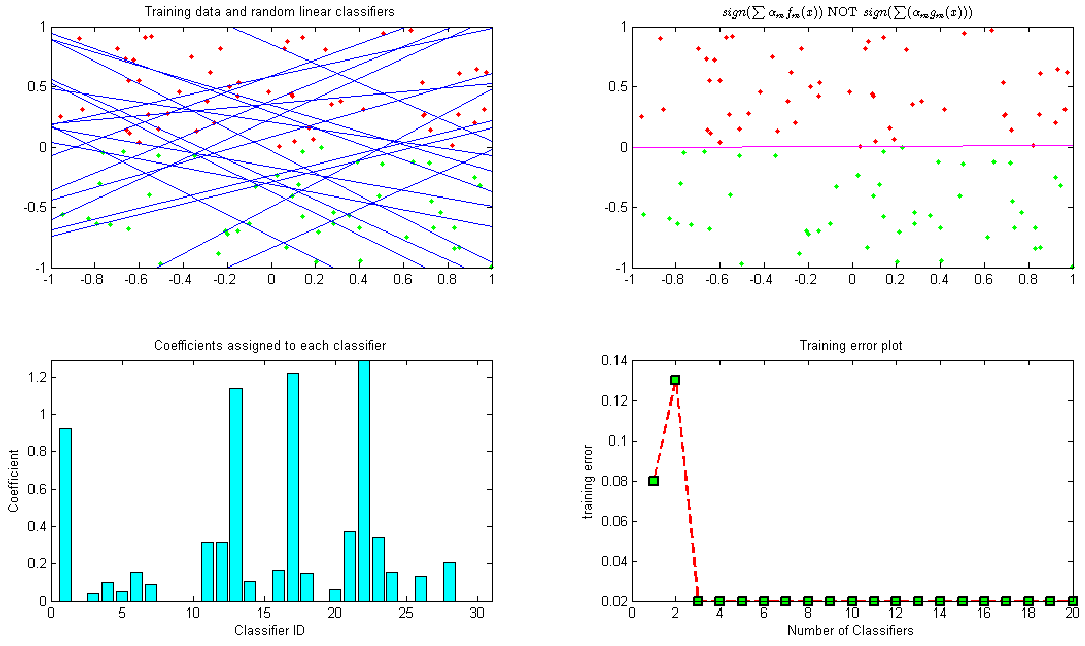
\includegraphics[scale=0.43]{images/AdaBoost_experiment}
\end{figure}
\end{frame}

\begin{frame}[allowframebreaks]\frametitle{Analysing Training Error}
Normalization constant at $t$-th iteration
\begin{equation}
\begin{array}{ll}
\mathcal{Z}_q&=\sum_{i=1}^Nw_i^{(q)}\exp(-y_i\alpha_i h_m(x_i))\\
&=\sum_{i:y_i\neq h_m(x_i)}w_i^{(q)}\exp(-y_i\alpha_i h_m(x_i))\\
&\quad+\sum_{i:y_i=h_m(x_i)}w_i^{(q)}\exp(-y_i\alpha_i h_m(x_i))\\
&=\epsilon_q\exp(-\alpha_q)+(1-\epsilon_q)\exp(\alpha_q)\\
&=2\sqrt{\epsilon_q (1-\epsilon_q)}\\
&=\sqrt{1-4\gamma_t^2}\leq \exp(-2\gamma_t^2)
\end{array}
\end{equation}
where \(\gamma_t=1/2-\epsilon_t\in [-1/2,1/2]\) measures how much better than random is $h_t$'s performance.

Weight for each sample after including $m$-th classifier into consideration
\begin{equation}
w_i^{(m+1)}=\frac{\exp(-y_i\sum_{q=1}^m\alpha_qh_q(x_i))}{N\prod_{q=1}^m\mathcal{Z}_q}=\frac{\exp(-y_if_m(x_i))}{N\prod_{q=1}^m\mathcal{Z}_q}
\end{equation}
\begin{equation}
h_m(x_i)\neq y_i\Rightarrow y_if_m(x_i)<0\Rightarrow\exp(-y_if_m(x_i))>1
\end{equation}
\begin{equation}
h_m(x_i)=y_i\Rightarrow y_if_m(x_i)>0\Rightarrow 0<\exp(-y_if_m(x_i))<1
\end{equation}
Upper bound of training error
\begin{equation}
\begin{array}{ll}
TrainingError&=\frac{1}{N}\sum_{i=1}^NI\{y_i\neq h_m(x_i)\}\\
&\leq\frac{1}{N}\sum_{i=1}^N\exp(-y_if_m(x_i))\\
&=\sum_{i=1}^Nw_i^{(m+1)}\prod_{q=1}^m\mathcal{Z}_q\\
&=\prod_{q=1}^m\mathcal{Z}_q\\
&=\prod_{q=1}^m\sqrt{1-4\gamma_t^2}\\
&\leq\exp(-2\sum_{q=1}^m\gamma_t^2)
\end{array}
\end{equation}
Therefore,if each as long as each weak classifier is slightly better or worse than random $\gamma_t>0$,then training error drops fast.
\end{frame}
\end{CJK*}
\end{document}
